\subsubsection{Raw Data}

\paragraph{Dendrograma de los clústeres obtenidos}

\begin{figure}[H]
    \centering
    
    \subfigure[\textit{HR}]{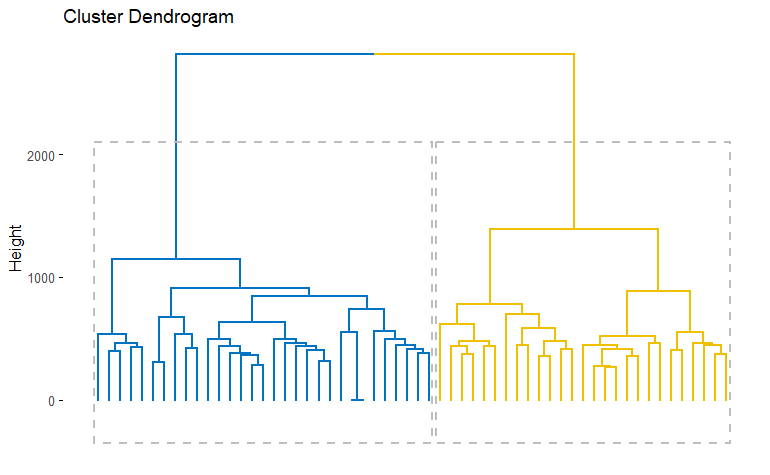
\includegraphics[width=0.45\textwidth]{img/01-1-eucl.png}}
    \subfigure[\textit{HR\_scaled}]{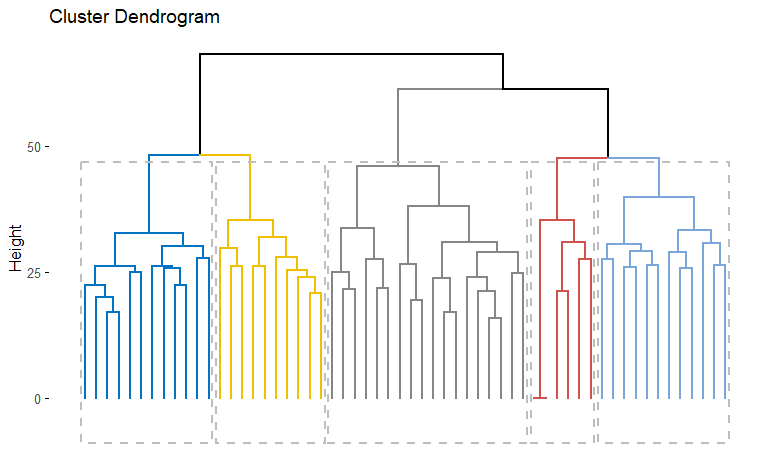
\includegraphics[width=0.45\textwidth]{img/02-1-eucl.png}}
    \subfigure[\textit{HR\_quantile}]{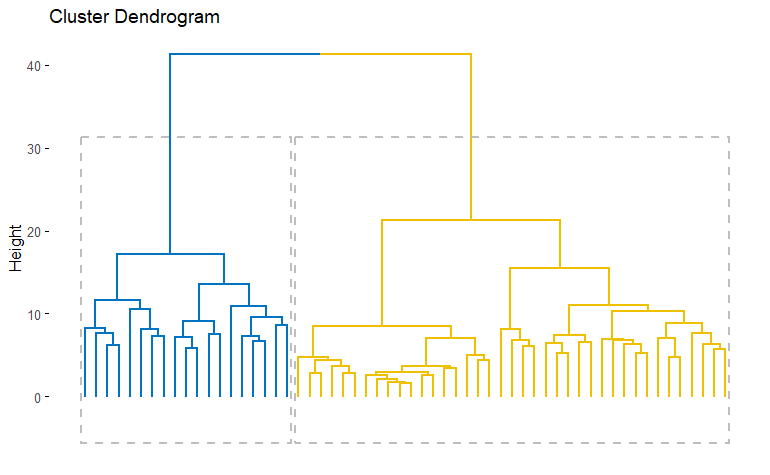
\includegraphics[width=0.5\textwidth]{img/03-1-eucl.png}}
    \caption{Dendogramas de \textit{HR}, \textit{HR\_scaled} y \textit{HR\_quantile}}
    \label{fig:raw_data_den_fc}
\end{figure}

\begin{figure}[ht]
    \centering
    \subfigure[\textit{SpO2}]{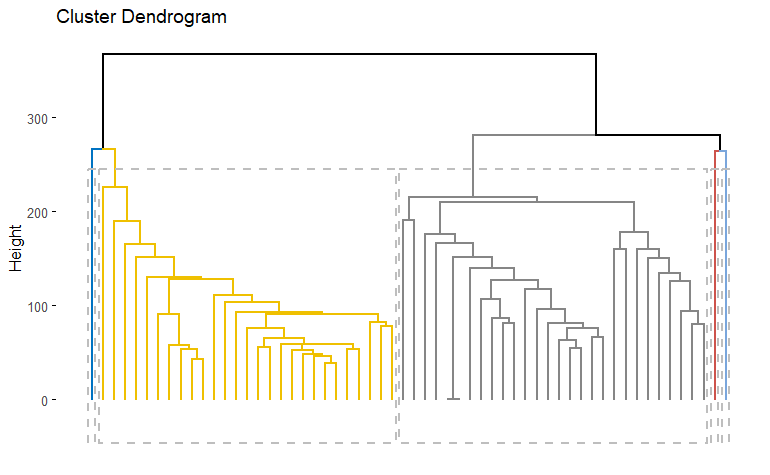
\includegraphics[width=0.5\textwidth]{img/04-1-eucl.png}}\hfill
    \subfigure[\textit{SpO2\_scaled}]{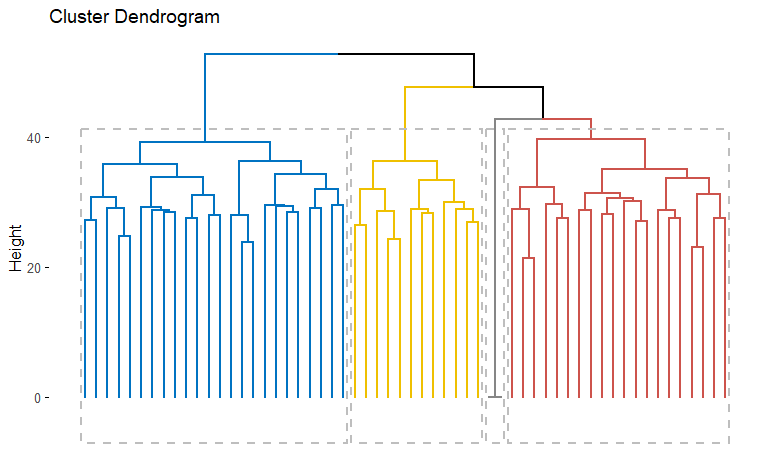
\includegraphics[width=0.5\textwidth]{img/05-1-eucl.png}}
    \caption{Dendogramas de \textit{SpO2} y \textit{SpO2\_scaled}}\label{fig:raw_data_den_spo2}
\end{figure}

\paragraph{Distribución de los clústeres obtenidos en función de las dos primeras componentes principales}

\begin{figure}[H]
    \centering
    \subfigure[\textit{HR}]{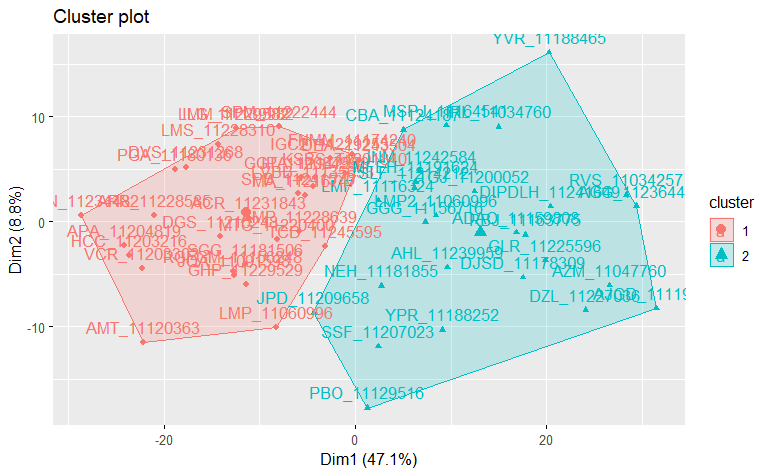
\includegraphics[width=0.45\textwidth]{img/01-2-eucl.png}}
    \subfigure[\textit{HR\_scaled}]{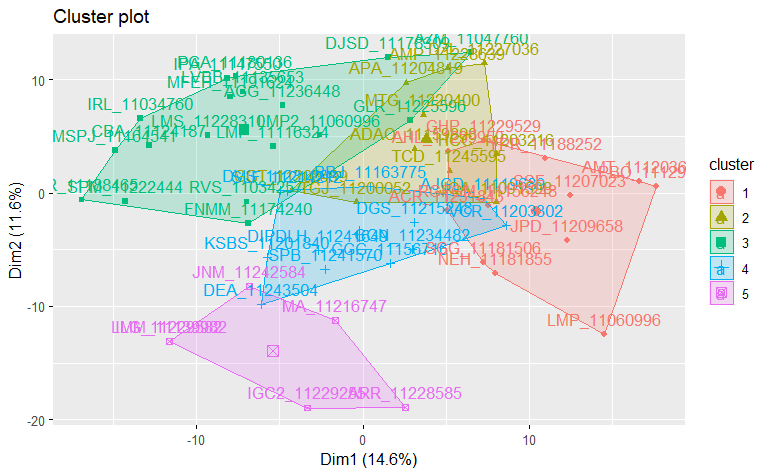
\includegraphics[width=0.45\textwidth]{img/02-2-eucl.png}}
    \subfigure[\textit{HR\_quantile}]{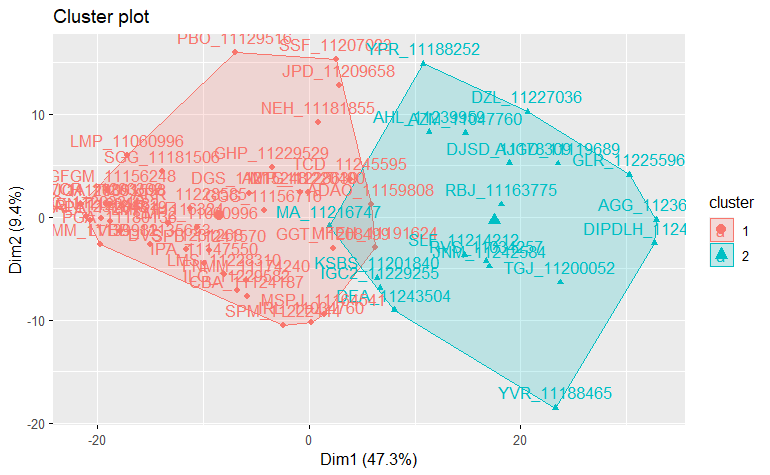
\includegraphics[width=0.5\textwidth]{img/03-2-eucl.png}}
    \caption{Cluster Plot de \textit{HR}, \textit{HR\_scaled} y \textit{HR\_quantile}}
    \label{fig:raw_data_pc_fc}
\end{figure}

\begin{figure}[ht]
    \centering
    \subfigure[\textit{SpO2}]{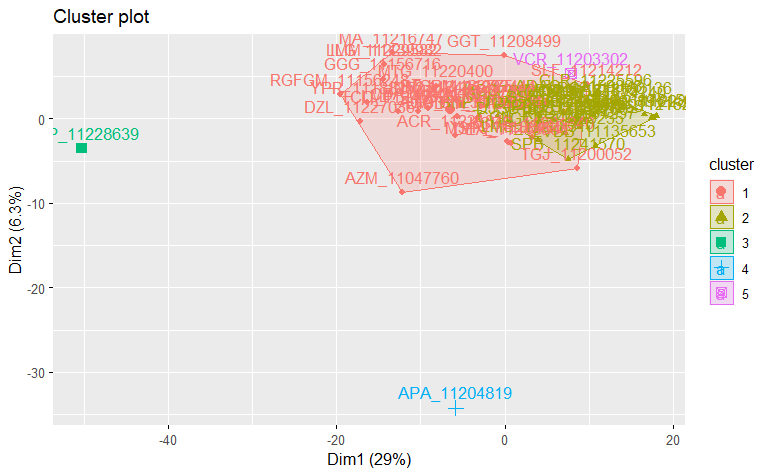
\includegraphics[width=0.5\textwidth]{img/04-2-eucl.png}}\hfill
    \subfigure[\textit{SpO2\_scaled}]{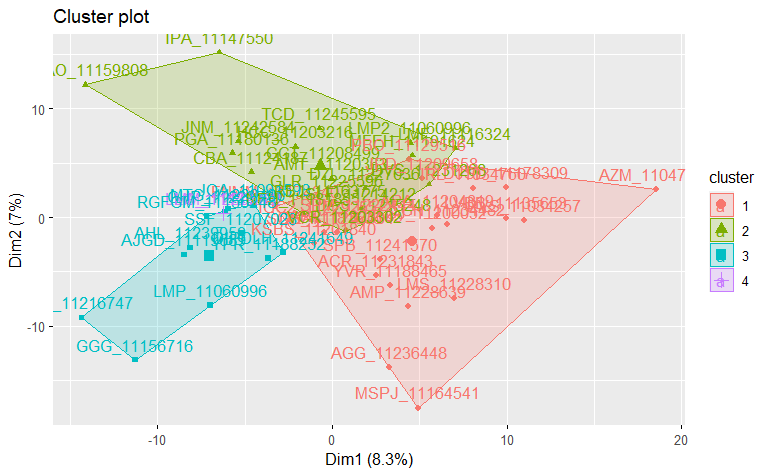
\includegraphics[width=0.5\textwidth]{img/05-2-eucl.png}}
    \caption{Cluster Plot de \textit{SpO2} y \textit{SpO2\_scaled}}\label{fig:raw_data_pc_spo2}
\end{figure}


\paragraph{Puntuación de Silhouette de los clústeres obtenidos}

\begin{figure}[H]
    \centering
    \subfigure[\textit{HR}]{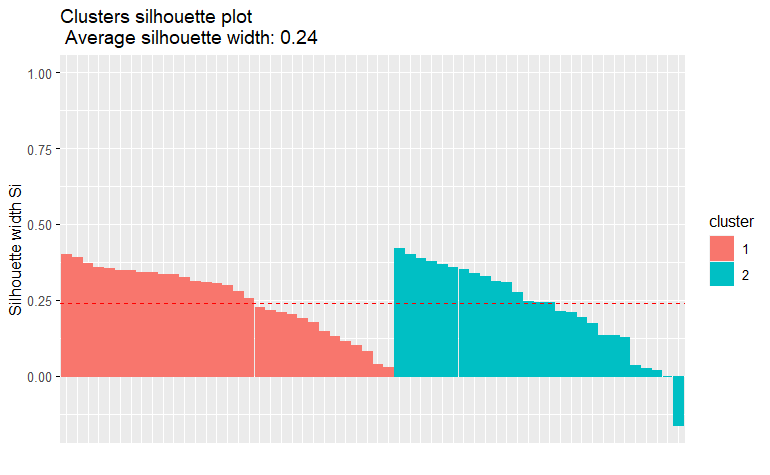
\includegraphics[width=0.45\textwidth]{img/01-3-eucl.png}}
    \subfigure[\textit{HR\_scaled}]{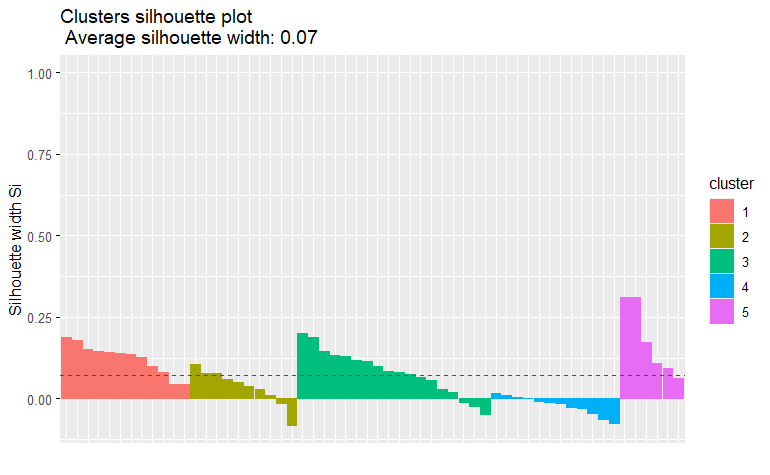
\includegraphics[width=0.45\textwidth]{img/02-3-eucl.png}}
    \subfigure[\textit{HR\_quantile}]{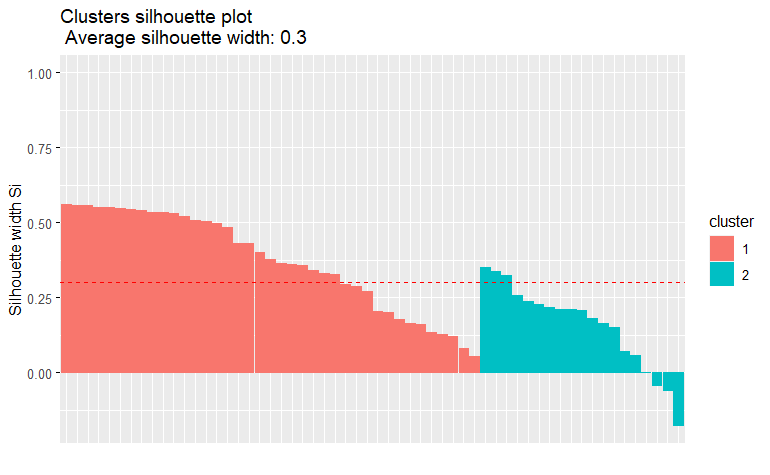
\includegraphics[width=0.5\textwidth]{img/03-3-eucl.png}}
    \caption{Silhouette Plot de \textit{HR}, \textit{HR\_scaled} y \textit{HR\_quantile}}\label{fig:raw_data_si_fc}
\end{figure}

\begin{figure}[ht]
    \centering
    \subfigure[\textit{SpO2}]{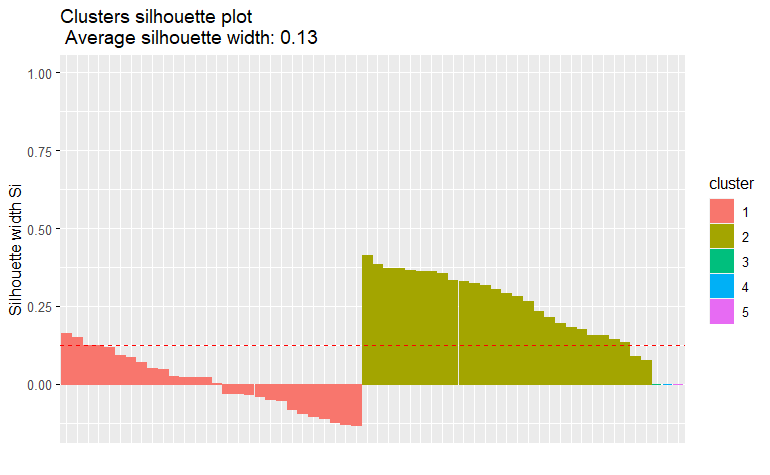
\includegraphics[width=0.5\textwidth]{img/04-3-eucl.png}}\hfill
    \subfigure[\textit{SpO2\_scaled}]{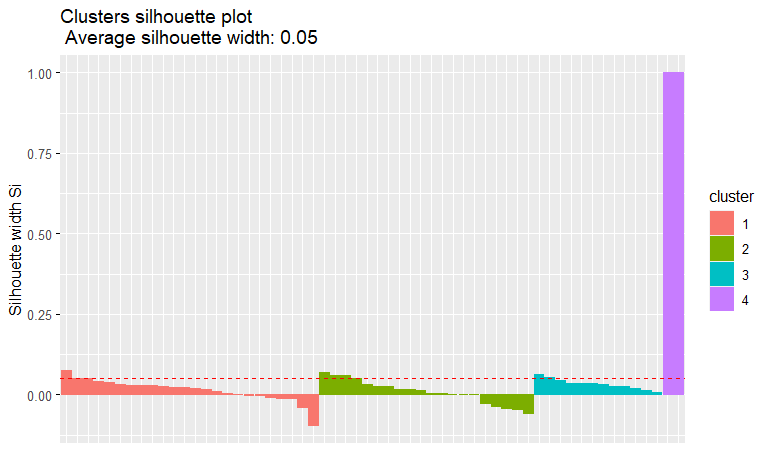
\includegraphics[width=0.5\textwidth]{img/05-3-eucl.png}}
    \caption{Silhouette Plot de \textit{SpO2} y \textit{SpO2\_scaled}}\label{fig:raw_data_si_spo2}
\end{figure}

\paragraph{Dendograma dividido en dos clústeres según los pacientes que han experimentado OAF}

\begin{figure}[H]
    \centering
    \subfigure[\textit{HR}]{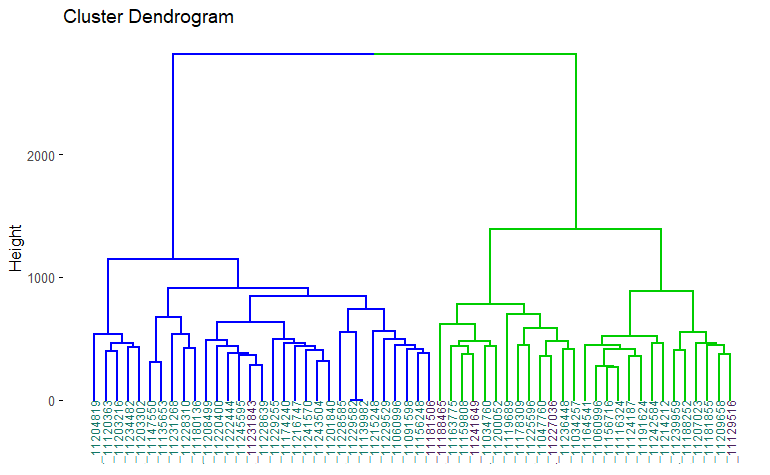
\includegraphics[width=0.45\textwidth]{img/01-4-eucl.png}}
    \subfigure[\textit{HR\_scaled}]{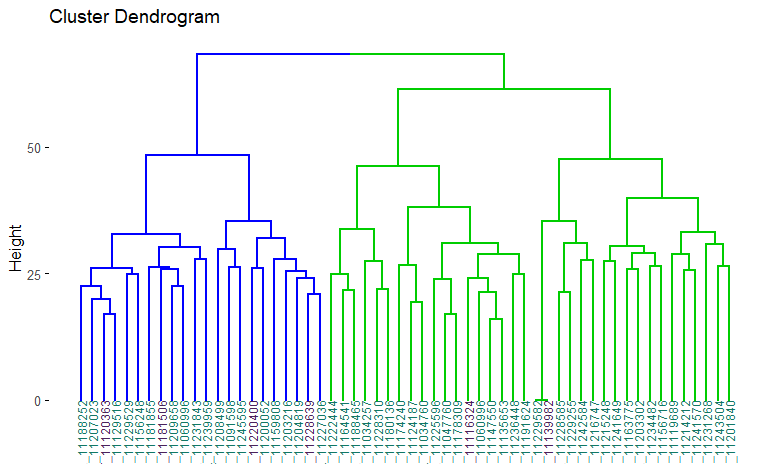
\includegraphics[width=0.45\textwidth]{img/02-4-eucl.png}}
    \subfigure[\textit{HR\_quantile}]{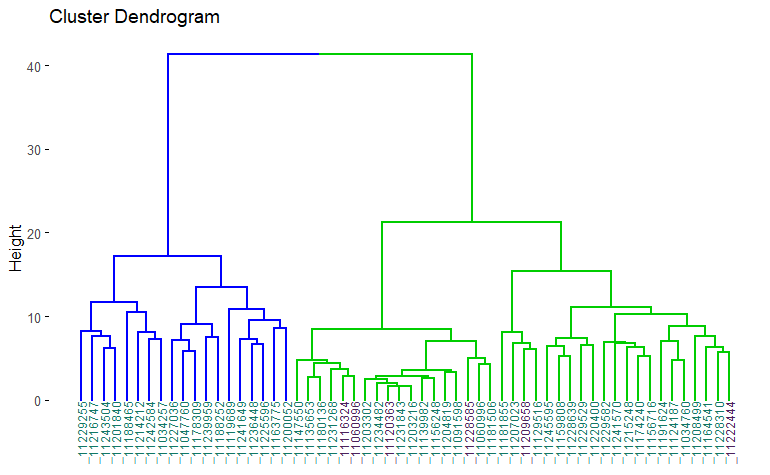
\includegraphics[width=0.5\textwidth]{img/03-4-eucl.png}}
    \caption{Dendograma Plot k = 2 de \textit{HR}, \textit{HR\_scaled} y \textit{HR\_quantile}}\label{fig:raw_data_ctg_fc}
\end{figure}

\begin{figure}[ht]
    \centering
    \subfigure[\textit{SpO2}]{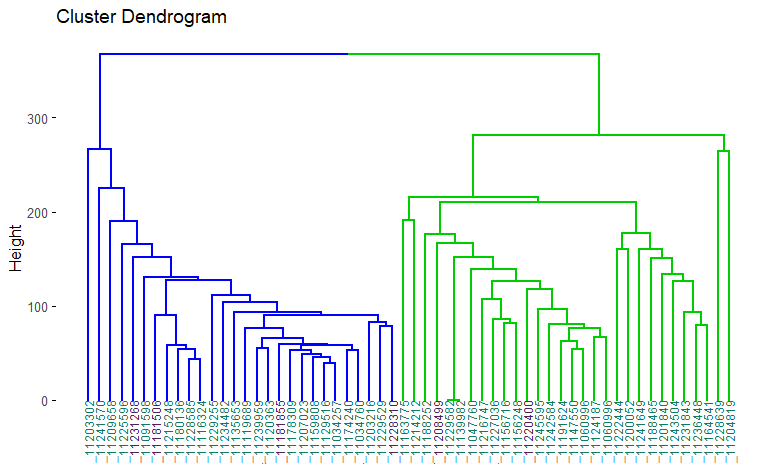
\includegraphics[width=0.5\textwidth]{img/04-4-eucl.png}}\hfill
    \subfigure[\textit{SpO2\_scaled}]{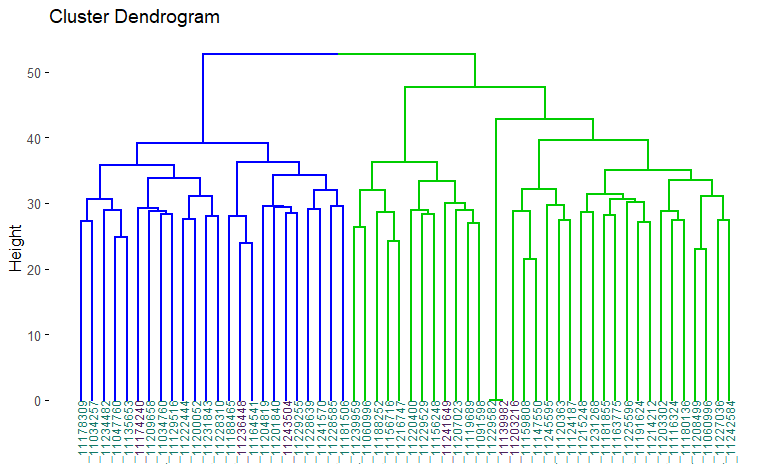
\includegraphics[width=0.5\textwidth]{img/05-4-eucl.png}}
    \caption{Dendograma Plot k = 2 de \textit{SpO2} y \textit{SpO2\_scaled}}\label{fig:raw_data_ctg_spo2}
\end{figure}

\paragraph{Clasificación mediente Random Forest de los clústeres según las variables \textit{Cuantitativas} y \textit{Cualitativas} de la Tabla~\ref{tabla:variables_estudio_final}}

\begin{figure}[H]
    \centering
    \begin{lstlisting}[frame=single, basicstyle=\small\ttfamily]
        randomForest(formula = CLUSTER ~ ., data = newSMOTE_EUCL) 
        Type of random forest: classification
              Number of trees: 500
No. of variables tried at each split: 5

 OOB estimate of  error rate: 39.66%
Confusion matrix:
1  2 class.error
1 19 12   0.3870968
2 11 16   0.4074074
    \end{lstlisting}
    \caption{Resultado de Random Forest para \textit{HR} utilizando variables \textit{Cuantitativas} y \textit{Cualitativas} de la Tabla~\ref{tabla:variables_estudio_final} y clasificación de clusters k = 2}\label{fig:random_forest_eucl_result_1}
\end{figure}
\begin{figure}[H]
    \centering
    \begin{lstlisting}[frame=single, basicstyle=\small\ttfamily]
        randomForest(formula = CLUSTER ~ ., data = newSMOTE_EUCL) 
               Type of random forest: classification
                     Number of trees: 500
No. of variables tried at each split: 5

        OOB estimate of  error rate: 43.1%
Confusion matrix:
  1  2 class.error
1 6 16   0.7272727
2 9 27   0.2500000
    \end{lstlisting}
    \caption{Resultado de Random Forest para \textit{HR\_scaled} utilizando variables \textit{Cuantitativas} y \textit{Cualitativas} de la Tabla~\ref{tabla:variables_estudio_final} y clasificación de clusters k = 2}
    \label{fig:random_forest_eucl_result_2}
\end{figure}

\begin{figure}[H]
    \centering
    \begin{lstlisting}[frame=single, basicstyle=\small\ttfamily]
        randomForest(formula = CLUSTER ~ ., data = newMWMOTE_EUCL) 
               Type of random forest: classification
                     Number of trees: 500
No. of variables tried at each split: 5

        OOB estimate of  error rate: 36.99%
Confusion matrix:
   1  2 class.error
1 26 13   0.3333333
2 14 20   0.4117647
    \end{lstlisting}
    \caption{Resultado de Random Forest para \textit{HR\_quantile} utilizando variables \textit{Cuantitativas} y \textit{Cualitativas} de la Tabla~\ref{tabla:variables_estudio_final} y clasificación de clusters k = 2}
    \label{fig:random_forest_eucl_result_3}
\end{figure}

\begin{figure}[H]
    \centering
    \begin{lstlisting}[frame=single, basicstyle=\small\ttfamily]
        randomForest(formula = CLUSTER ~ ., data = newSMOTE_EUCL) 
               Type of random forest: classification
                     Number of trees: 500
No. of variables tried at each split: 5

        OOB estimate of  error rate: 48.28%
Confusion matrix:
   1  2 class.error
1 16 14   0.4666667
2 14 14   0.5000000
    \end{lstlisting}
    \caption{Resultado de Random Forest para \textit{SpO2} utilizando variables \textit{Cuantitativas} y \textit{Cualitativas} de la Tabla~\ref{tabla:variables_estudio_final} y clasificación de clusters k = 2}\label{fig:random_forest_eucl_result_4}
\end{figure}
\begin{figure}[H]
    \centering
    \begin{lstlisting}[frame=single, basicstyle=\small\ttfamily]
        randomForest(formula = CLUSTER ~ ., data = newSMOTE_EUCL) 
               Type of random forest: classification
                     Number of trees: 500
No. of variables tried at each split: 5

        OOB estimate of  error rate: 55.17%
Confusion matrix:
   1  2 class.error
1  6 18   0.7500000
2 14 20   0.4117647
    \end{lstlisting}
    \caption{Resultado de Random Forest para \textit{SpO2\_scaled} utilizando variables \textit{Cuantitativas} y \textit{Cualitativas} de la Tabla~\ref{tabla:variables_estudio_final} y clasificación de clusters k = 2}
    \label{fig:random_forest_eucl_result_5}
\end{figure}

\paragraph{Mean Decrease Accuracy de las 5 primeras variables descriptivas utilizadas en Random Forest}

\begin{table}[H]
    \centering
    \begin{tabular}{lr}
        \toprule
        \textbf{Variable} & \textbf{Mean Decrease Accuracy} \\
        \midrule
        PESO & 3.4318174 \\
        SCORE\_WOOD\_DOWNES\_INGRESO & 3.3955906 \\
        EDAD & 3.2490817 \\
        SCORE\_CRUCES\_INGRESO & 2.5964057 \\
        FR\_0\_8h & 1.9810445 \\
        \bottomrule
    \end{tabular}
    \caption{Mean Decrease Accuracy \textit{HR}}
\end{table}

\begin{table}[H]
    \centering
    \begin{tabular}{lr}
        \toprule
        \textbf{Variable} & \textbf{Mean Decrease Accuracy} \\
        \midrule
        FR\_0\_8h & 3.2107589 \\
        SCORE\_CRUCES\_INGRESO & 2.8801769 \\
        SCORE\_WOOD\_DOWNES\_INGRESO & 2.8575468 \\
        PESO & 2.3468291 \\
        EDAD & 2.3045016 \\
        \bottomrule
    \end{tabular}
    \caption{Mean Decrease Accuracy \textit{HR\_scaled}}
\end{table}

\begin{table}[H]
    \centering
    \begin{tabular}{lr}
        \toprule
        \textbf{Variable} & \textbf{Mean Decrease Accuracy} \\
        \midrule
        SCORE\_WOOD\_DOWNES\_INGRESO & 3.8597355 \\
        SCORE\_CRUCES\_INGRESO & 3.3423195 \\
        PESO & 3.2757830 \\
        DIAS\_O2\_TOTAL & 2.8530298 \\
        FR\_0\_8h & 2.6567973 \\
        \bottomrule
    \end{tabular}
    \caption{Mean Decrease Accuracy \textit{HR\_quantile}} 
\end{table}

\begin{table}[H]
    \centering
    \begin{tabular}{lr}
        \toprule
        \textbf{Variable} & \textbf{Mean Decrease Accuracy} \\
        \midrule
        SCORE\_WOOD\_DOWNES\_INGRESO & 3.5645422 \\
        FR\_0\_8h & 2.7355615 \\
        PESO & 2.6841347 \\
        SCORE\_CRUCES\_INGRESO & 2.6712216 \\
        EDAD & 2.3318932 \\
        \bottomrule
    \end{tabular}
    \caption{Mean Decrease Accuracy \textit{SpO2}}
\end{table}

\begin{table}[H]
    \centering
    \begin{tabular}{lr}
        \toprule
        \textbf{Variable} & \textbf{Mean Decrease Accuracy} \\
        \midrule
        SCORE\_WOOD\_DOWNES\_INGRESO & 3.8160260 \\
        FR\_0\_8h & 2.8111591 \\
        PESO & 2.3188373 \\
        SCORE\_CRUCES\_INGRESO & 2.2545591 \\
        EDAD & 2.1933961 \\
        \bottomrule
    \end{tabular}
    \caption{Mean Decrease Accuracy \textit{SpO2\_scaled}}
\end{table}


\paragraph{Clasificación mediente Random Forest de los clústeres según Raw Data utilizada para genear los mismos} 

\begin{figure}[H]
    \centering
    \begin{lstlisting}[frame=single, basicstyle=\small\ttfamily]
        randomForest(formula = CLUSTER ~ ., data = data_frame_merge_EUCL) 
               Type of random forest: classification
                     Number of trees: 500
No. of variables tried at each split: 21

        OOB estimate of  error rate: 6.9%
Confusion matrix:
   1  2 class.error
1 29  2  0.06451613
2  2 25  0.07407407
    \end{lstlisting}
    \caption{Resultado de Random Forest para \textit{HR} utilizando Raw Data y clasificación de clusters k = 2}\label{fig:random_forest_eucl_result_RF_1}
\end{figure}
\begin{figure}[H]
    \centering
    \begin{lstlisting}[frame=single, basicstyle=\small\ttfamily]
        randomForest(formula = CLUSTER ~ ., data = data_frame_merge_EUCL) 
               Type of random forest: classification
                     Number of trees: 500
No. of variables tried at each split: 21

        OOB estimate of  error rate: 15.52%
Confusion matrix:
   1  2 class.error
1 15  7  0.31818182
2  2 34  0.05555556
    \end{lstlisting}
    \caption{Resultado de Random Forest para \textit{HR\_scaled} utilizando Raw Data y clasificación de clusters k = 2}
    \label{fig:random_forest_eucl_result_RF_2}
\end{figure}

\begin{figure}[H]
    \centering
    \begin{lstlisting}[frame=single, basicstyle=\small\ttfamily]
        randomForest(formula = CLUSTER ~ ., data = data_frame_merge_EUCL) 
               Type of random forest: classification
                     Number of trees: 500
No. of variables tried at each split: 21

        OOB estimate of  error rate: 5.17%
Confusion matrix:
   1  2 class.error
1 39  0   0.0000000
2  3 16   0.1578947
    \end{lstlisting}
    \caption{Resultado de Random Forest para \textit{HR\_quantile} utilizando Raw Data y clasificación de clusters k = 2}
    \label{fig:random_forest_eucl_result_RF_3}
\end{figure}

\begin{figure}[H]
    \centering
    \begin{lstlisting}[frame=single, basicstyle=\small\ttfamily]
        randomForest(formula = CLUSTER ~ ., data = data_frame_merge_EUCL) 
               Type of random forest: classification
                     Number of trees: 500
No. of variables tried at each split: 21

        OOB estimate of  error rate: 15.52%
Confusion matrix:
   1  2 class.error
1 25  5   0.1666667
2  4 24   0.1428571
    \end{lstlisting}
    \caption{Resultado de Random Forest para \textit{SpO2} utilizando Raw Data y clasificación de clusters k = 2}\label{fig:random_forest_eucl_result_RF_4}
\end{figure}
\begin{figure}[H]
    \centering
    \begin{lstlisting}[frame=single, basicstyle=\small\ttfamily]
        randomForest(formula = CLUSTER ~ ., data = data_frame_merge_EUCL) 
               Type of random forest: classification
                     Number of trees: 500
No. of variables tried at each split: 21

        OOB estimate of  error rate: 25.86%
Confusion matrix:
   1  2 class.error
1 15  9   0.3750000
2  6 28   0.1764706
    \end{lstlisting}
    \caption{Resultado de Random Forest para \textit{SpO2\_scaled} utilizando Raw Data y clasificación de clusters k = 2}
    \label{fig:random_forest_eucl_result_RF_5}
\end{figure}

\paragraph{Distribución de la Importancia de Raw Data}

\begin{figure}[H]
    \centering
    \subfigure[\textit{HR}]{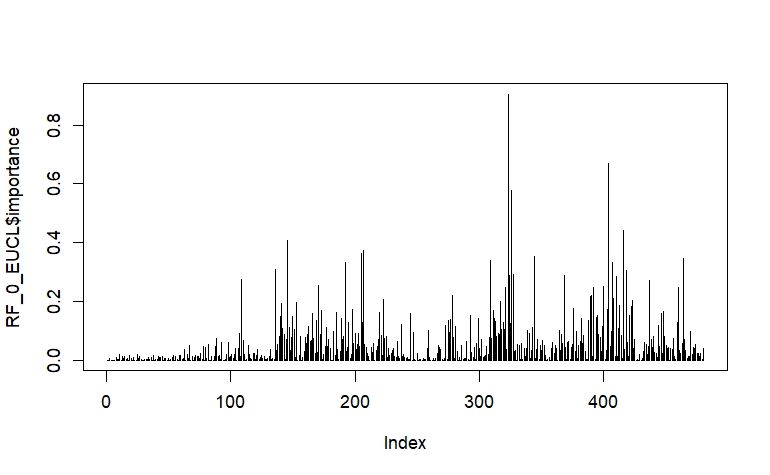
\includegraphics[width=0.45\textwidth]{img/01-5-eucl.png}}
    \subfigure[\textit{HR\_scaled}]{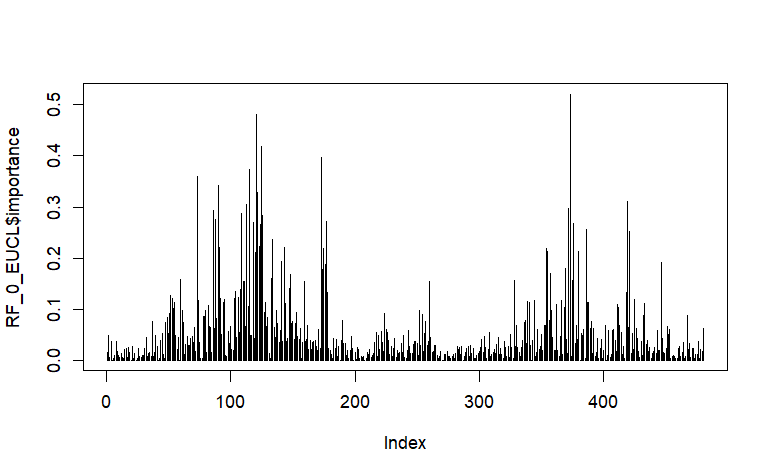
\includegraphics[width=0.45\textwidth]{img/02-5-eucl.png}}
    \subfigure[\textit{HR\_quantile}]{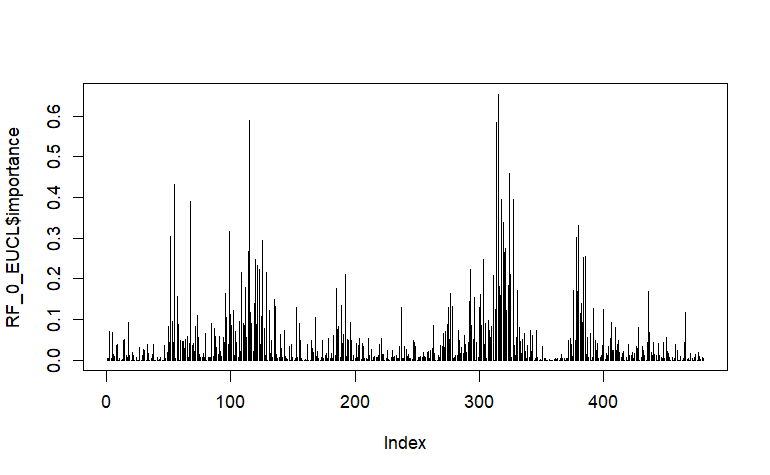
\includegraphics[width=0.5\textwidth]{img/03-5-eucl.png}}
    \caption{Importancia Raw Data de \textit{HR}, \textit{HR\_scaled} y \textit{HR\_quantile}}\label{fig:raw_data_imp_fc}
\end{figure}

\begin{figure}[ht]
    \centering
    \subfigure[\textit{SpO2}]{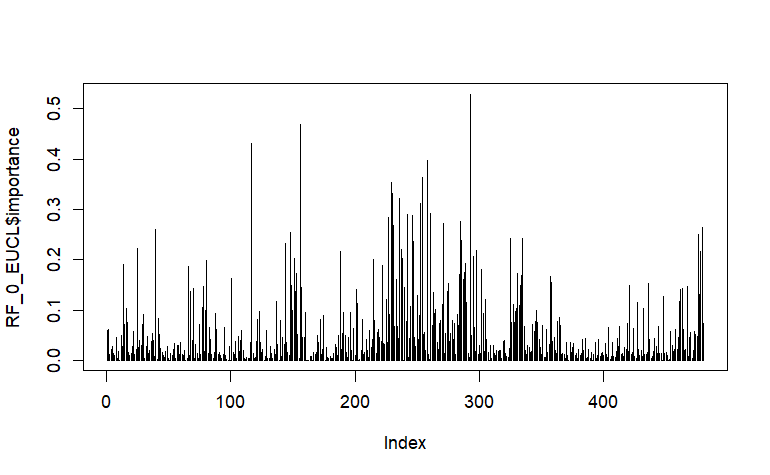
\includegraphics[width=0.5\textwidth]{img/04-5-eucl.png}}\hfill
    \subfigure[\textit{SpO2\_scaled}]{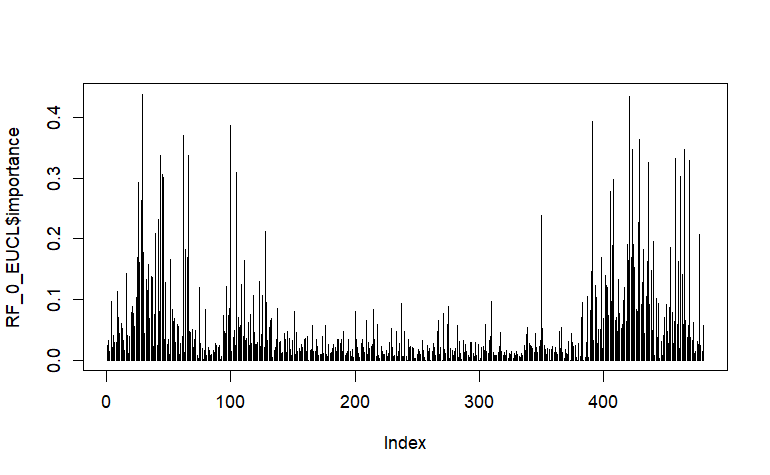
\includegraphics[width=0.5\textwidth]{img/05-5-eucl.png}}
    \caption{Importancia Raw Data de \textit{SpO2} y \textit{SpO2\_scaled}}\label{fig:raw_data_imp_spo2}
\end{figure}


\paragraph{Media de los valores de Raw Data en función de los clusters generados $k = 2$}

\begin{figure}[H]
    \centering
    \subfigure[\textit{HR}]{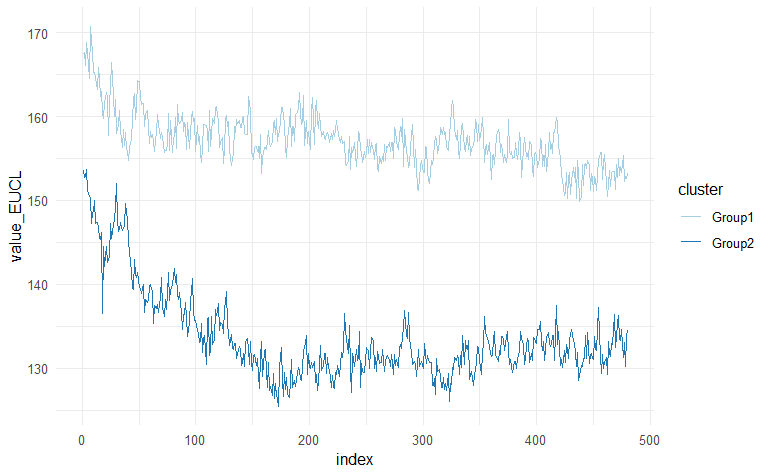
\includegraphics[width=0.45\textwidth]{img/01-6-eucl.png}}
    \subfigure[\textit{HR\_scaled}]{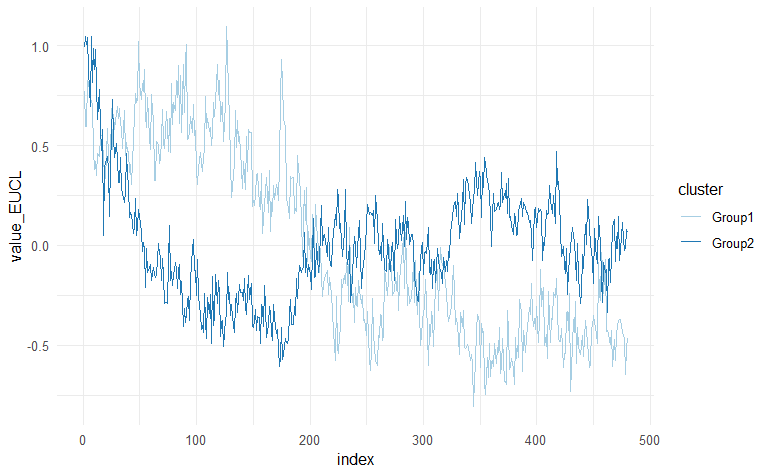
\includegraphics[width=0.45\textwidth]{img/02-6-eucl.png}}
    \subfigure[\textit{HR\_quantile}]{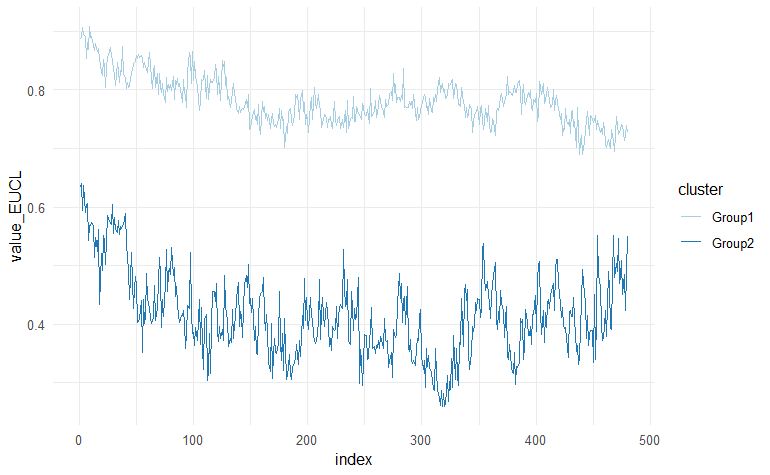
\includegraphics[width=0.5\textwidth]{img/03-6-eucl.png}}
    \caption{Valores de Raw Data por cluster k = 2 de \textit{HR}, \textit{HR\_scaled} y \textit{HR\_quantile}}\label{fig:raw_data_cls_fc}
\end{figure}

\begin{figure}[ht]
    \centering
    \subfigure[\textit{SpO2}]{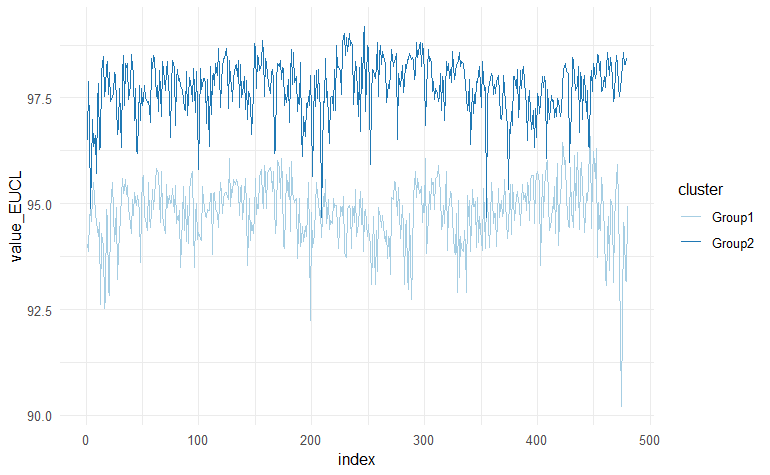
\includegraphics[width=0.5\textwidth]{img/04-6-eucl.png}}\hfill
    \subfigure[\textit{SpO2\_scaled}]{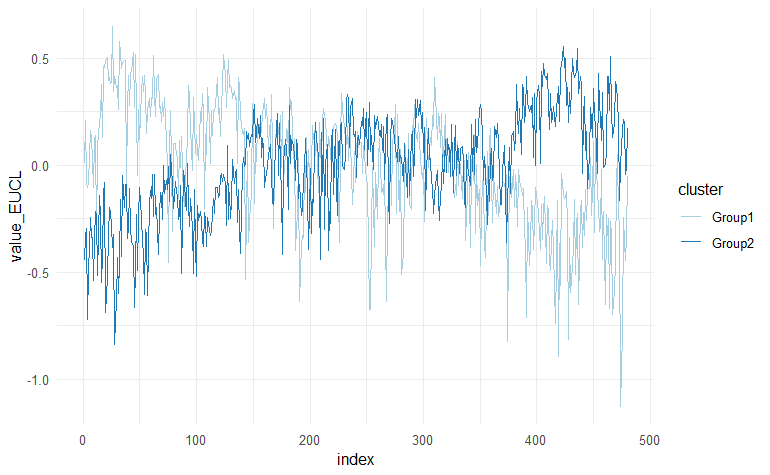
\includegraphics[width=0.5\textwidth]{img/05-6-eucl.png}}
    \caption{Valores de Raw Data por cluster k = 2 de \textit{SpO2} y \textit{SpO2\_scaled}}\label{fig:raw_data_cls_spo2}
\end{figure}
